\subsection{实验设计说明}
为了验证本文提出的基于自编码降维的特征工程对最终分类结果的实际有效性,整个实验设计将分别使用两份数据集,并在相同参数的模型上分别进行验证和对比:

\begin{itemize}
    \item 使用常见的WOE编码、IV值筛选、特征交叉组合的特征工程处理之后的数据集
    \item 经过简单处理和WOE编码后,再利用神经网络自编码器(Auto-Encoder)进行非线性降维和特征提取后的数据集
\end{itemize}

\subsection{实验模型介绍}
如下图所示,本文采用的模型基本思路为:先通过初步特征工程和WOE编码,得到13个基本特征$x$;将这13个基本特征输入Auto-encoder神经网络模型,分别进行13维$\rightarrow$3维的特征压缩和3维$\rightarrow$13维的特征还原,还原后的结果记为$\hat x$\\

将还原前后的$x$和$\hat x$之间的差距作为神经网络的损失函数,即$Loss = \sum\limits_i (x_i-\hat x_i)^2$,对损失函数进行梯度下降,训练出一个能够稳定将13维特征压缩到3维特征的神经网络自编码器。最后,提取出隐藏层的3维特征,作为特征工程的最终结果。

\begin{figure}[H]
    \centering
    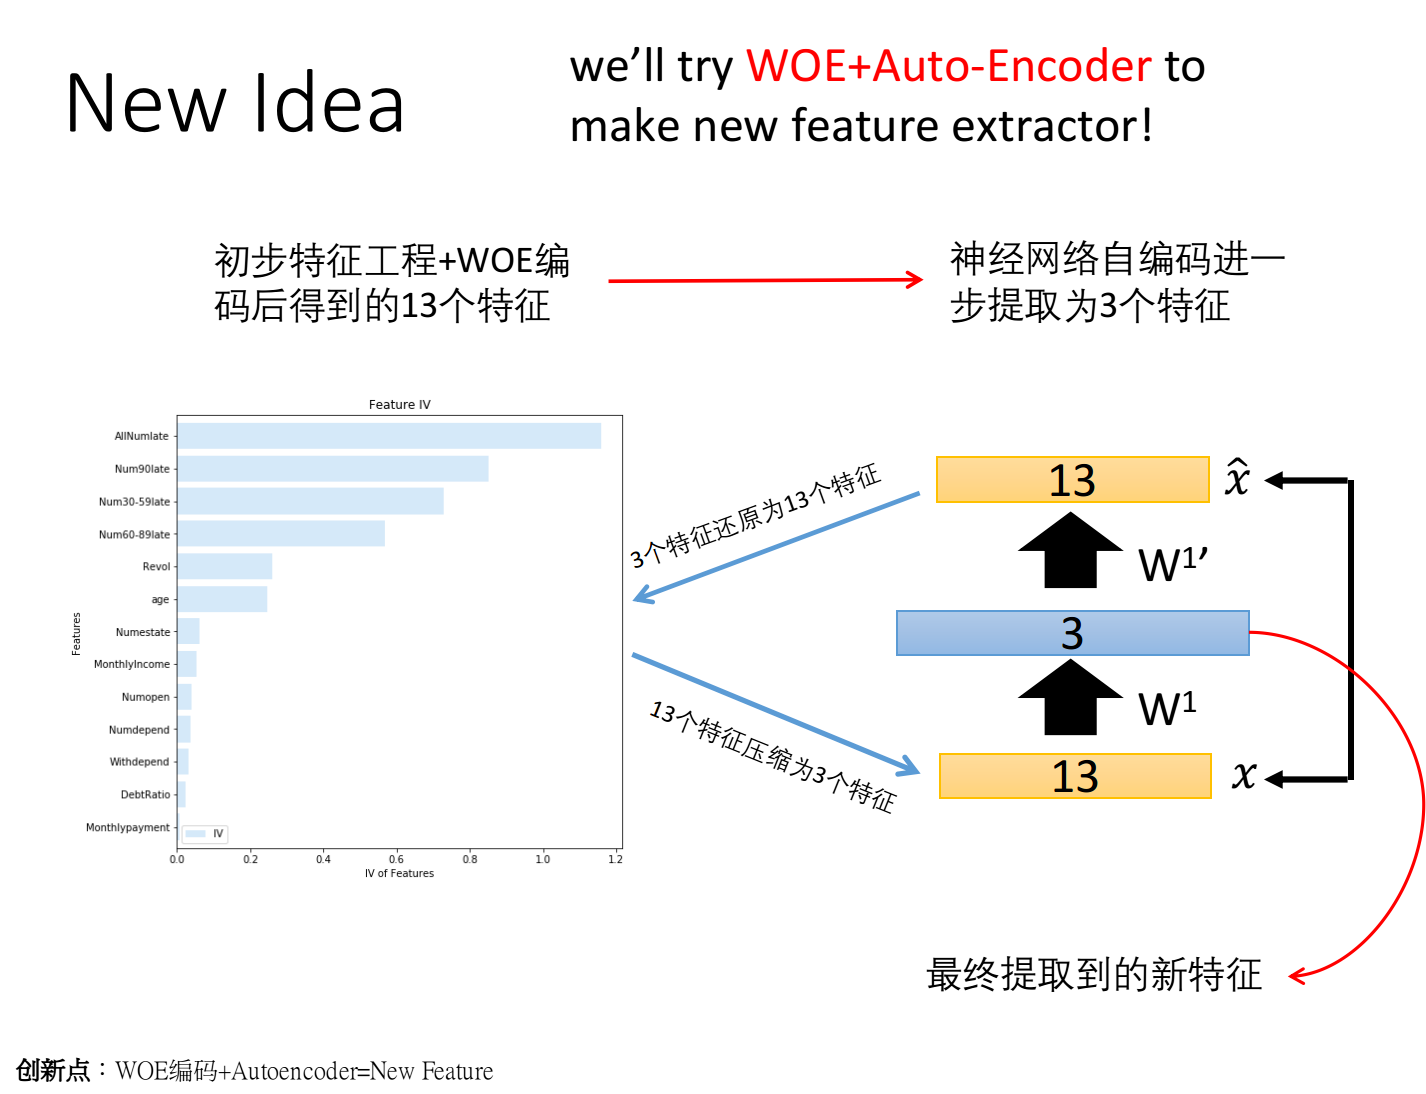
\includegraphics[width=0.7\linewidth]{idea.png}
    \caption{自编码模型简介}
    \label{fig:idea}
\end{figure}

\subsection{模型算法实现}
特征处理模型算法实现主要分为两部分,WOE编码和Auto-encoder特征提取。

实现数据分箱、WOE编码的关键算法如下:
\begin{lstlisting}[frame=shadowbox]
    def bin_woe(tar, var, n=None, cat=None):
    """
    连续自变量分箱,woe,iv变换
    tar:target目标变量
    var:进行woe,iv转换的自变量
    n:分组数量
    """
    total_bad = tar.sum()
    total_good =tar.count()-total_bad
    totalRate = total_good/total_bad
    
    if cat == 's':
        msheet = pd.DataFrame({tar.name:tar,var.name:var,'var_bins':pd.qcut(var, n, duplicates='drop')})
        grouped = msheet.groupby(['var_bins'])
    elif (cat == 'd') and (n is None):
        msheet = pd.DataFrame({tar.name:tar,var.name:var})
        grouped = msheet.groupby([var.name])
        
    groupBad = grouped.sum()[tar.name]
    groupTotal = grouped.count()[tar.name]
    groupGood = groupTotal - groupBad
    groupRate = groupGood/groupBad
    groupBadRate = groupBad/groupTotal
    groupGoodRate = groupGood/groupTotal

    woe = np.log(groupRate/totalRate)
    iv = np.sum((groupGood/total_good-groupBad/total_bad)*woe)
    
    if cat == 's':
        new_var, cut = pd.qcut(var, n, duplicates='drop',retbins=True, labels=woe.tolist())
    elif cat == 'd':
        dictmap = {}
        for x in woe.index:
            dictmap[x] = woe[x]
        new_var, cut = var.map(dictmap), woe.index

    return woe.tolist(), iv, cut, new_var
\end{lstlisting}

PyTorch实现Auto-encoder自编码器的模型如下:

模型训练使用参数: EPOCH=100,lr=0.001,Loss=MSE
\begin{lstlisting}[frame=shadowbox]
    class AutoEncoder(nn.Module):
    def __init__(self):
        super(AutoEncoder, self).__init__()
        
        self.encoder = nn.Sequential(
            nn.Linear(13, 64),
            nn.Tanh(),
            nn.Linear(64, 32),
            nn.Tanh(),
            nn.Linear(32, 3)
        )
        
        self.decoder = nn.Sequential(
            nn.Linear(3, 32),
            nn.Tanh(),
            nn.Linear(32, 64),
            nn.Tanh(),
            nn.Linear(64, 13)
        )
        
    def forward(self, x):
        encode = self.encoder(x)
        decode = self.decoder(encode)
        return encode, decode
\end{lstlisting}



\subsection{自编码结果可视化分析}
为了更直观地感受基于自编码降维的特征工程的效果,这里将降维后的三个维度可视化在三维空间上。下图是5万个样本点根据降维后的三个坐标绘制出来的图像,展示了两个方向上样本点的分布。

\begin{figure}[H]
    \centering
    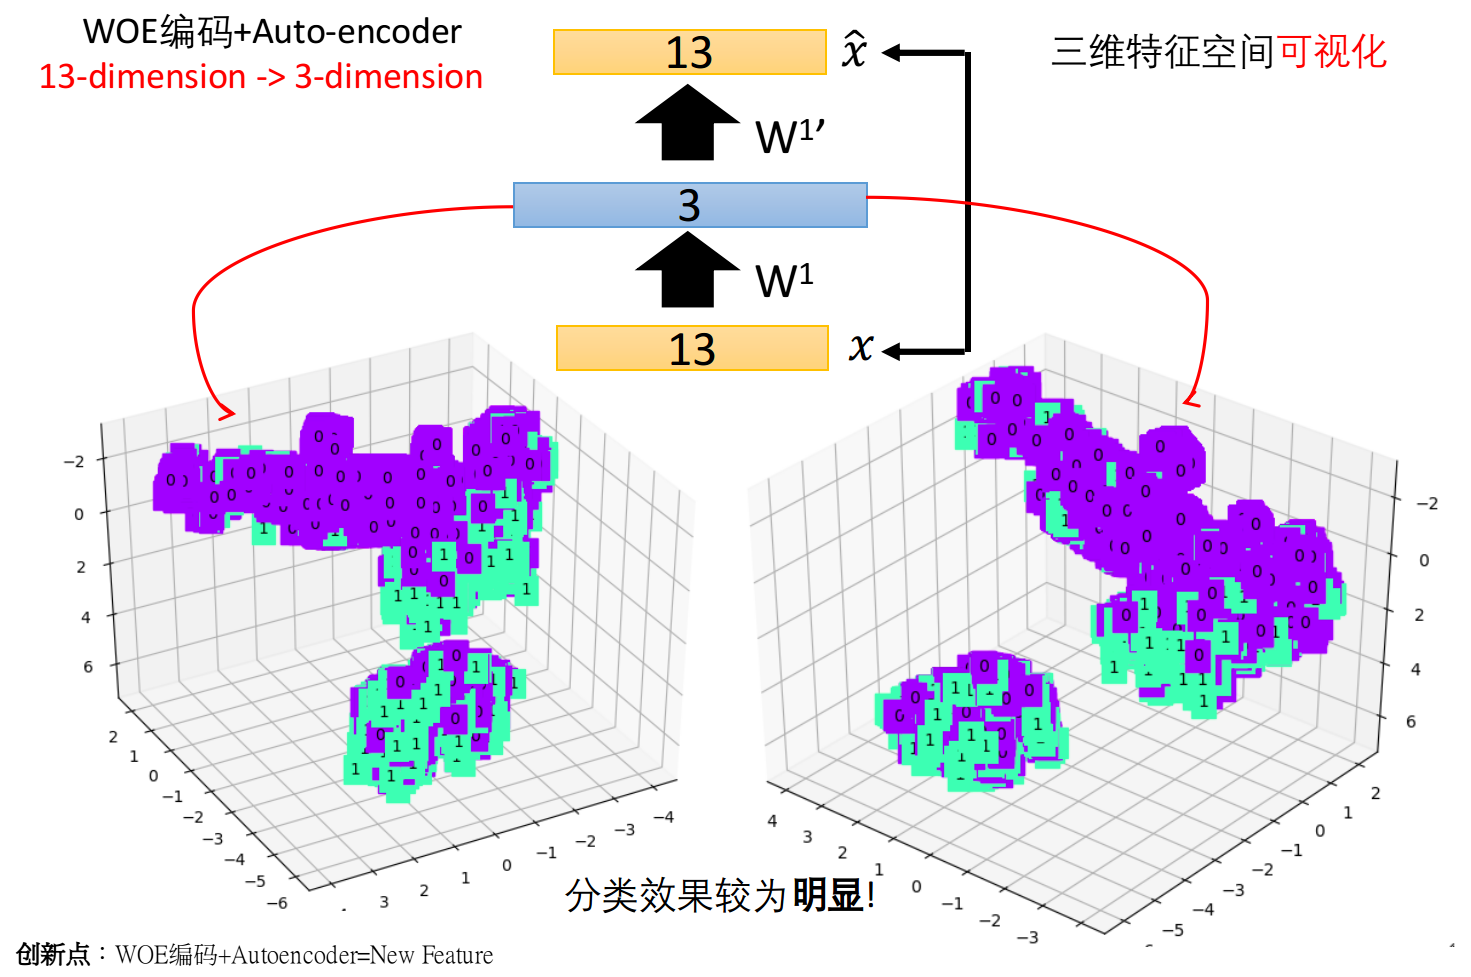
\includegraphics[width=0.7\linewidth]{visual.png}
    \caption{自编码特征结果可视化}
    \label{fig:visual}
\end{figure}

可以清楚地看到,通过该模型获取到的3-dimension feature具备较好的分类能力,能够使两个不同类别的样本点较为明显地分布在空间的两块不同区域。该实验结果表明,本文提出的方法确实具备一定的可行性,能够在一定程度上提高分类效果。\\

除了定性分析之外,接下来将定量对比分析“是否使用自编码提取特征”在相同分类模型上所表现出来的AUC值情况,来进一步证明该方法的正确性。

\subsection{不同分类器上的对比}
